% Source: Code/CommonSenseCarolina/latex/usc-cost-pressure.tex
% Description: Out-of-state tuition grew slower than inflation overall, but began accelerating in 2023--24 \citep{CollegeTuitionCompare2025

\documentclass[border=4pt]{standalone}
\usepackage{graphicx}
\usepackage{pgfplots}
\usepackage{tikz}
\usepackage{xcolor}
\pgfplotsset{compat=1.18}

\definecolor{Garnet}{HTML}{73000A}
\definecolor{Atlantic}{HTML}{466A9F}
\definecolor{Congaree}{HTML}{1F414D}
\definecolor{Rose}{HTML}{CC2E40}
\definecolor{Black90}{HTML}{363636}
\definecolor{Black50}{HTML}{A2A2A2}
\definecolor{Black10}{HTML}{ECECEC}


\begin{document}
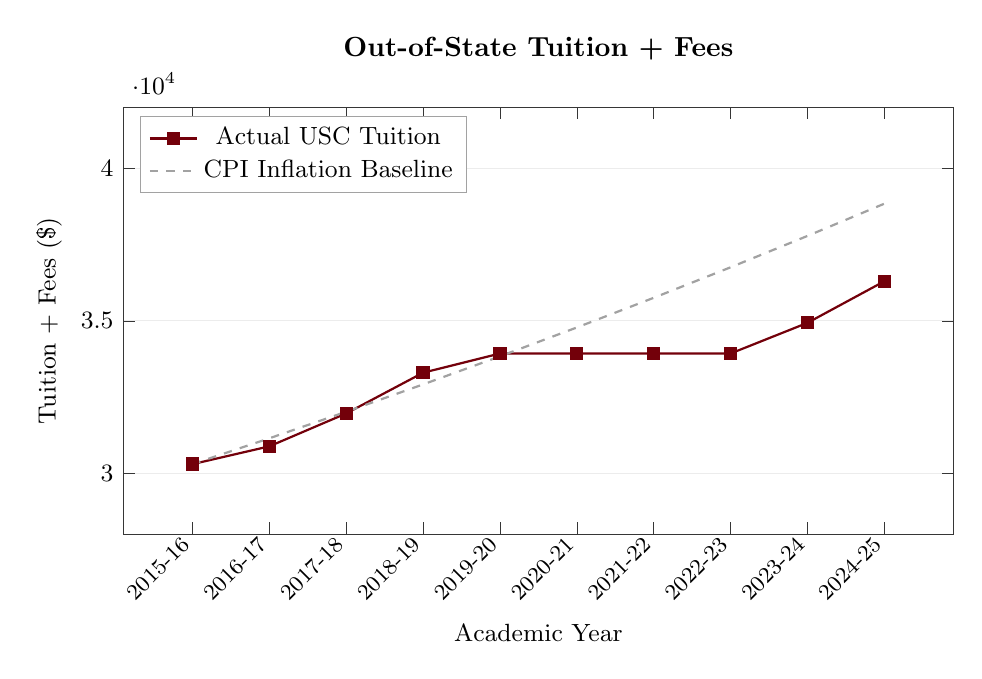
\begin{tikzpicture}
\begin{axis}[
    width=\textwidth,
    height=7cm,
    xlabel={Academic Year},
    ylabel={Tuition + Fees (\$)},
    xlabel style={font=\small},
    ylabel style={font=\small},
    xticklabel style={font=\footnotesize, rotate=45, anchor=east},
    yticklabel style={font=\small},
    symbolic x coords={2015-16,2016-17,2017-18,2018-19,2019-20,2020-21,2021-22,2022-23,2023-24,2024-25},
    xtick=data,
    ymin=28000, ymax=42000,
    ymajorgrids=true,
    grid style={color=Black10},
    axis line style={color=Black90},
    tick style={color=Black90},
    legend style={at={(0.02,0.98)}, anchor=north west, font=\small, draw=Black50},
    title={\textbf{Out-of-State Tuition + Fees}},
    title style={font=\normalsize, at={(0.5,1.05)}},
]
\addplot[color=Garnet, thick, mark=square*, mark size=2] coordinates {
    (2015-16,30298) (2016-17,30882) (2017-18,31962) (2018-19,33298)
    (2019-20,33928) (2020-21,33928) (2021-22,33928) (2022-23,33928)
    (2023-24,34934) (2024-25,36298)
};
\addplot[color=Black50, thick, dashed, mark=none] coordinates {
    (2015-16,30298) (2016-17,31146) (2017-18,32017) (2018-19,32914)
    (2019-20,33835) (2020-21,34782) (2021-22,35756) (2022-23,36757)
    (2023-24,37786) (2024-25,38844)
};
\legend{Actual USC Tuition, CPI Inflation Baseline}
\end{axis}
\end{tikzpicture}
\end{document}
